\documentclass[12pt]{article}
\usepackage{amsfonts,amssymb}
\usepackage{amsmath}
\usepackage{hyperref}
\usepackage{graphicx}
\usepackage{listings}
%\documentstyle[12pt,amsfonts]{article}
%\documentstyle{article}

\setlength{\topmargin}{-.5in}
\setlength{\oddsidemargin}{0 in}
\setlength{\evensidemargin}{0 in}
\setlength{\textwidth}{6.5truein}
\setlength{\textheight}{8.5truein}
%
%\input ../adgeomcs/lamacb.tex
%\input mac.tex
%\input mathmac.tex
%
\input xy
\xyoption{all}
\def\fseq#1#2{(#1_{#2})_{#2\geq 1}}
\def\fsseq#1#2#3{(#1_{#3(#2)})_{#2\geq 1}}
\def\qleq{\sqsubseteq}
%cis51109hw1

%
\begin{document}
\begin{center}
\fbox{{\Large\bf Set Operations}}\\
\vspace{1cm}
\end{center}


\medskip\noindent
	

\vspace{0.5cm}\noindent

\section*{Common mistakes}

One of the common mistakes in set theory is to confuse `element of' and `subset of'. Confuse $\in$ and $\subset$.

Is it $2 \in \{1,2,3\}$ or $2 \subset \{1,2,3\}$? - 2 is just a number. It is not a set. It is an element of the set.

Is it $\{2\} \in \{1,2,3\}$ or $\{2\} \subset \{1,2,3\}$? - Now $\{2\}$ represents a set. Is this set completely contained inside the set $\{1,2,3\}$. Yes. Therefore we have a subset in this case.

It gets more interesting (or confusing :)) when you are dealing with sets of sets.

Is $\{2\} \in \{\{2\},\{3\}\}$? Yes! Because, in this example, the set's individual elements are sets themselves.

So what would be a subset of the set above? - $\{\{2\}\}$ would be one example. There are 3 more subsets. What are they?

\section*{More unions and intersections}

Set unions and intersections are not restricted to just 2 sets. In fact, expressing operations with 3 sets using Venn diagrams is quite easy.

In general a 3 set Venn diagram will look something like this.

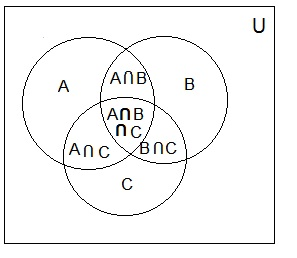
\includegraphics{3setsVenn.png}

Using just the Venn diagram, these properties can be clearly demonstrated.

\begin{itemize}
\item Commutative laws

$A \cap B = B \cap A$ and $A \cup B = B \cup A$

\item Associative laws

$(A \cap B) \cap C = A \cap (B \cap C)$ and $(A \cup B) \cup C = A \cup (B \cup C)$

\item Distributive laws

$A \cap (B \cup C) = (A \cap B) \cup (A \cap C)$ and $A \cup (B \cap C) = (A \cup B) \cap (A \cup C)$
\end{itemize}

Very often when wanting to express a number of sets, we use subscripts. 
Generally, each individual set will have something to do with the subscript.

Examples

\begin{enumerate}
\item Let $N_i$ represent the positive integers that are divisible by $i$. Then

$N_4 = \{4,8,12,\ldots\}$
$N_{11} = \{11, 22, 33, \ldots\}$

\item Let $B_i$ represent the set $\{i,-i\}$. Then $B_2 = \{2,-2\}$.
\end{enumerate}

If you have a collection of sets, it becomes convenient to introduce notation for the union and intersection.

$\displaystyle \bigcup_{i=1}^n A_i$ - union of the sets $A_1$ through $A_n$.

$\displaystyle \bigcap_{i=1}^n A_i$ - intersection of the sets $A_1$ through $A_n$.

Assume $P_i$ is used to represent all the people in the world who are $i$ years old. 
Then something like $\displaystyle \bigcup_{i=0}^{130} P_i$ would give you all the people in the world since no one is older than 130. 

In the same example, note that $P_i \cap P_j = \emptyset$, for any pair of $i \neq j$. After all, no one can be both $i$ years old and $j$ years old if the $i$ and $j$ are distinct.

\section*{Cartesian Product}

$A \times B$, called the cartesian product of A and B consists of ordered pairs of the form (a,b) where $a \in A$ and $b \in B$.

Say $A = \{1,2,3\}$ and $B = \{2,5\}$ then the Cartesian product is

$A \times B = \{(1,2), (1,5), (2,2), (2,5), (3,2), (3,5)\}$ 

Common mistake:- In general the Cartesian product operator is not commutative. That means $B \times A \neq A \times B$. Why? Because the order matters!

Note that the Cartesian product produces another {\bf set}. But the elements of the set are pairs. 

\medskip

If you have seen coordinate geometry then it should be easy to see that coordinates of the form (x, y) are just elements of the set $\mathbb{R}^2$. 

\section*{Generalized Cartesian products}

The Cartesian product can be applied to more than two sets as well. Consider a sequence of n sets, $A_1, A_2, \ldots, A_n$. The elements of the Cartesian product of $A_1, A_2, \ldots, A_n$ are ordered sequences of $n$ entries, called n-tuples. The ith entry in each n-tuple is an element of $A_i$. The Cartesian product of $A_1, A_2, \ldots, A_n$, denoted $A_1 \times A_2 \times \ldots \times A_n$, is defined to be:

$A_1 \times A_2 \times \ldots \times A_n = \{ (a_1, a_2, \ldots , a_n) : a_i \in A_i \text{ for all integers } i \text{ such that } 1 \le i \le n\}$

In general, the idea of a Cartesian product is extremely useful when you want to refer to ordered groupings. If you have to make a sandwich where you first pick bread from a set like $B = \{\text{white},\text{wheat}\}$ and pick cheese from a set like 
$C = \{\text{edam}, \text{camembert}\}$ then every sandwich can be expressed as an ordered pair of the form (bread, cheese). So how many possible sandwiches are there? 

The number of sandwiches is the same as $|B \times C| = 2 \times 2 = 4$.

\vspace{1cm}

Notation:- As with `usual' math, $P \times P \times P$ is often denoted by $P^3$.
\vspace{1cm}

If $|A| = 2$ and $|B| = 4$, how many elements does $A \times B$ have?

The Cartesian product will pair each element with $A$ with each element of $B$. For the first element of $A$, it gets paired with each one of the 4 elements of $B$. For the second element of $A$, it gets paired with each one of the 4 elements of $B$. So it is $ 2 \times 4 = 8$.

In general, if you take the cross product of a set with cardinality $m$ and a set with cardinality $n$, you get a set of cardinality $mn$.

\section*{Partitioning a set}

A set $A$ is set to be partitioned by a family of subsets of $A$, $A_1, A_2, \ldots, A_n$ if the following are satisfied

$\displaystyle A = \bigcup_{i=1}^n A_i$ and

$\displaystyle A_i \cap A_j = \emptyset \text{ for every } i \neq j$. This condition is also called being mutually disjoint.

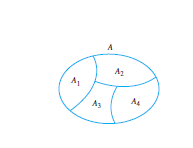
\includegraphics{partition.png}

Why is this useful?

If you know that a set $A$ is partitioned by $A_i, 1 \le i \le n$, then we can easily deduce that

$\displaystyle |A| = \sum_{i=1}^n |A_i|$.

Example

Let $A = \{1,2,3,4,5,6\} \text{ and } A_1 = \{1,2\}, A_2 = \{3,4\} \text{ and } A_3 = \{5,6\}$. Is $\{A_1, A_2, A_3\}$ a partition of $A$.

Yes. 

Is $\{\{a,d,e\},\{b,c\},\{d,f\}\}$ a partition of $\{a,b,c,d,e,f\}$?

No. $d$ is in two of the sets.



\section*{Application of Cartesian products}

Databases - The JOIN syntax in databases is fundamentally using Cartesian products.

Example taken from \href{http://en.wikipedia.org/wiki/Join\_(SQL)}{http://en.wikipedia.org/wiki/Join\_(SQL)}

\section*{Application of partitions}

One of the first steps in designing a parallel program is to break the problem into discrete "chunks" of work that can be distributed to multiple tasks. This is known as decomposition or partitioning.

Often useful for counting things as we will see soon.

\end{document}



